Um die oben genannten Spiele um einen virtuellen Teil erweitern zu k�nnen werden Features ben�tigt. Eine von uns getroffene Auswahl wird im folgenden beschrieben. 

\section{Erweiterte Realit�t}
Features, die explizit die Realit�t erweitern und dadurch einen Mehrwert zum Spiel beitragen.


\subsection*{Integration virtueller Objekte in die physische Umgebung}\label{sec:integration-virtueller-objekte-in-die-physische-umgebung}
Um ein virtuelles Spiel in die physische Umgebung integrieren zu k�nnen, m�ssen auch alle Objekte des virtuellen Spieles in die physische Umgebung gebracht werden. Dies kann z.B. auf einer virtuellen Karte, die die Wirklichkeit widerspiegelt, geschehen.

Beispiele f�r solche Objekte sind z.B. die Items bei unserem Spiel Snake, die es einzusammeln gilt und die auf einer Karte auf dem Smartphone dargestellt und in unserem Fall zuf�llig innerhalb eines erreichbaren Radius um unsere Spieler platziert werden. Ein anderes Beispiel sind feste Spieler-Basen, die bei Spielen wie unserer Capture-the-Flag-Abwandlung zum Einsatz kommen. Virtuelle Objekte k�nnen auch Startpunkte f�r Teams sein. 
Dabei bietet sich an, diese auf eine relativ freie Fl�che zu setzen. Generell sollte darauf geachtet werden, dass die Objekte nicht innerhalb eines Geb�udes platziert werden, da der GPS-Sensor in Geb�uden nur sehr ungenaue bis gar keine Ergebnisse liefert und Objekte in nicht zug�nglichen R�umen/Geb�uden nicht erreicht werden k�nnen, au�er indem man die Reichweite der Interaktion sehr gro� setzt. Das gilt auch f�r anderes unerreichbares Terrain wie Berge, Seen, Meere oder einfach gesperrte Bereiche wie Vorg�rten oder Truppen�bungspl�tze.


Dies kann mit Hilfe der folgenden technischen L�sungen umgesetzt werden. Die Kartendarstellung (s. \ref{kartendarstellung}) hilft enorm die Objekte in die physische Welt einzuarbeiten, da sie lediglich auf der Karte eingef�gt werden m�ssen. Mit der Kollisionsabfrage (s. \ref{kollisionsabfrage}) kann eine Kollision zweier Objekte, zum Beispiel eine "`Snake"' mit einem "`Item"', verwirklicht werden. 

%Die Positionsabfrage wird unter anderem daf�r ben�tigt um sicherzustellen, dass das Objekt in der N�he des Spielers erstellt wird. (s. \ref{positionsermittlung}).

\subsection*{Darstellung der physischen und virtuellen Umgebung}\label{sec:darstellung-der-physischen-und-virtuellen-umgebung}

Die physische Welt in eine virtuelle Umgebung zu �bertragen kann einen enormen Mehrwert des Spiels darstellen.
Sei es in einer Karte als �bersicht oder lediglich eine Anzeige ob man sich innerhalb bzw. au�erhalb des Spielfelds befindet. Des weiteren kann mit den heutigen Smartphones auch wie in  Abbildung \ref{fig:aug01} gezeigt eine Augmented Reality geschaffen werden, die die Darstellung der realen Welt um etwa die Beschriftung der zu sehenden Gesch�fte erweitert.
\begin{figure}[htbp]
  \centering
    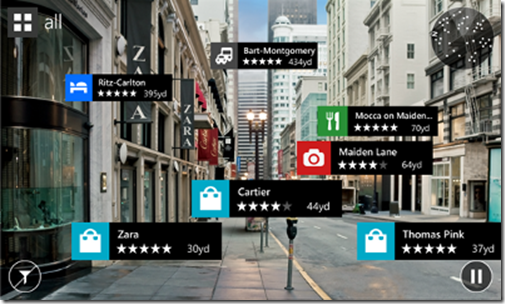
\includegraphics[width=0.9\textwidth]{3-Spielkonzepte/3-1-Erweiterte_Realitaet/map01.png}
    
		\caption{Handyscreen um die zu sehenden Gesch�fte, Hotels, etc. erweitert
	(Quelle: \url{http://blogs.bing.com/maps/wp-content/uploads/sites/3/2013/06/clip_5F00_image006_5F00_thumb_5F00_4AEFDB0C.png})
		}
		\label{fig:aug01} 
\end{figure}
 Hierf�r werden Kartendarstellung (s. \ref{kartendarstellung}) und Positionsermittlung (s. \ref{positionsermittlung}) ben�tigt.

\subsection*{Kollision virtueller Objekte}\label{sec:kollision-virtueller-objekte}
Treffen zwei virtuelle Objekte aufeinander kann ein Event ausgel�st werden. Wird bei Snake z.B. der eigene Schwanz ber�hrt, was laut der Regeln nicht erlaubt ist, muss dies dem Spieler mitgeteilt werden und evtl. weitere Ereignisse ausgef�hrt werden.

Dazu werden die Kollisionsabfrage (s. \ref{kollisionsabfrage}) und die  Positionsermittlung (s. \ref{positionsermittlung}) gebraucht.


\subsection*{Einsammeln von Objekten}\label{sec:einsammeln-von-objekten}
Eine Variante der Kollision mit virtuellen Objekten ist das Einsammeln. Wenn ein Spieler in Reichweite eines Items ist, das es einzusammeln gilt, kann dies entweder automatisch passieren oder �ber eine Aufforderung auf dem mobilen Ger�t. Zur Best�tigung, dass etwas eingesammelt wurde, kann nun wiederum ein akustisches oder haptisches Signal gegeben werden.

 Erreicht werden kann dies durch die Positionsermittlung (s. \ref{positionsermittlung}) und die Kollisionsabfrage (s. \ref{kollisionsabfrage}). 
 
 %F�r weitere Best�tigungssignale sind auch andere Sensorik (s. \ref{sensorik}) von Vorteil.
